%Document vide aux normes de l'École nationale des Chartes
%Dernières modifications E. Rouquette (12/2023)

\part{Partie 1 : Historique et enjeux de la découvrabilité}
\chapter{Aux origines était la Disponibilité}

\subsection{La nouvelle bibliothèque de Babel : vers un Big data patrimonial}

Depuis plus de vingt ans, les institutions patrimoniales ont massivement numérisé leurs collections. Si l’utopie de recréation d’une « Bibliothèque d’Alexandrie 2.0 » s’est rapidement révélée irréaliste\footcite[p. 20]{bermes2024}, il n’en reste pas moins que le volume de données numérisées est devenu colossal. Cela est encore plus vrai dans le domaine du patrimoine audiovisuel : les institutions occidentales se sont retrouvées, au tournant des années 2000, face à des problématiques de dégradations des supports très importantes, notamment à cause du tristement célèbre « syndrome du vinaigre »\footnote{« Le syndrome du vinaigre est le phénomène de dépolymérisation spontanée qui se produit dans les films pour la photographie ou le cinéma, par dégradation de l’acétate en acide acétique, causant ainsi la détérioration du support des œuvres. » - Wikipédia, Syndrome du vinaigre}. Il a donc fallu numériser ; mais la dégradation des supports n’est pas la seule raison de ces programmes de numérisation massifs, et il nous semble ici intéressant de détailler les autres. En premier lieu, il faut évoquer qu'ils ont eu lieu à une période où la société elle-même se « numérisait » : il y a eu une demande forte de la part des citoyens d’accès à ce qu’ils considéraient comme « leur patrimoine »\footcite{rezzonico2023}; qui plus est — dans le cas de la RTS — la mise à disposition de quelques fragments de la collection avait créé un engouement qui a permis de donner une impulsion au programme de numérisation ; il faut ensuite ajouter à cela un besoin d’accès multiple aux mêmes documents, c’est le cas à la RTS évidemment (plusieurs émissions avaient souvent besoin de réutiliser les mêmes images d’illustration), mais c’est encore plus le cas pour des documents tels que l’État civil, massivement numérisé par les archives départementales en France. Pour terminer, et c’est loin d’être anodin, il faut ajouter à toutes ces raisons le fait que « c’était possible »\footcite{barcella2024a} : l’arrivée de technologies de stockage de masse (LTO)\footnote{Pour linear tape open, méthode de stockage magnétique permettant de stocker de grands volumes de données de façon plus pérenne que sur disque dur} et de chaînes de numérisation plus rapides et efficaces rendaient la numérisation réalisable et soutenable financièrement. Ce mouvement qui a eu lieu dans les institutions audiovisuelles est un exemple assez extrême : peu d’institutions ont numérisé la totalité de leur patrimoine même si la volonté de le faire n’a pas manqué. Elle s’est heurtée à la réalité des métiers et à l’intérêt d’une telle opération\footcite[p. 21]{bermes2024}.

Loin d’être les seules à produire des données massives\index{Données massives}, les institutions patrimoniales suivent le mouvement initié par les géants du web, et notamment Google qui en 2005 annonce à la foire du livre de Francfort le projet « Ocean » qui vise à numériser intégralement les collections de six puis seize bibliothèques partenaires\footcite{ertzscheid2019}, créant un véritable électrochoc qui a marqué l'intensification des volumes numérisés pour tous les acteurs, privés ou publics.\footcite{bermes2024}.

Les données disponibles sur le web, au tournant des années 2010, deviennent donc massives. S’il est très délicat de donner des chiffres sur ce volume, qui de toute manière sont inintelligibles, on estime généralement qu’en 2010 1,2 zettaoctet\footnote{Un zettaoctet correspond à un million de téraoctets (To) ou un milliard de gigaoctets(Go)} ont été produits contre 64 Zo en 2020 et sur ce même volume, environ 5\% seraient conservés soit 3,2 Zo\footcite{zotero-284}. Le secteur patrimonial est loin d’être responsable de cette augmentation, c’est plutôt l’essor du web dit 2.0 : celui des blogs, des réseaux sociaux, de l’interactivité\footcite{zotero-283} décrit en 2009 par Benjamin Bayard dans une phrase qui est devenue célèbre : « L’imprimerie a permis au peuple de lire, internet va lui permettre d’écrire » à qui il faut imputer cette production documentaire massive (suivi de nos jours par les objets connectés). Cette surabondance documentaire sans précédent pose évidemment des questions de découvrabilité, et plus encore de recherchabilité. De fait, dès 2007, un article intitulé « The discoverability of the web »\footcite{dasgupta2007} pose la question du pourcentage de pages renvoyées par un moteur de recherche sur un sujet donné par rapport aux sources utiles : face à la masse grandissante de contenus sur le web, comment garantir la pertinence et l’efficacité des moteurs de recherche ? C’est bien là un signe que l’enjeu de découvrabilité n’est pas intrinsèque au secteur public et patrimonial.

Dans tous les cas, les volumes de données sont tels qu’on peut parler, dans notre cas de \textit{big data patrimonial}\index{Big data} : 10 millions de documents sur Gallica, la bibliothèque numérique de la Bibliothèque nationale de France\footcite{zotero-281}, 53 millions sur Européana\footcite{zotero-280}, portail\index{Portail} européen regroupant les bibliothèques numériques du continent, 1 million d’heures de programmes numérisés à la RTS\footcite{sonderegger2024}, 28 millions à l’Institut national de l’audiovisuel (INA) totalisant 80 pétaoctets de données\footcite{alquier2024}. Il devient totalement impossible pour l’humain d’appréhender les collections numérisées de façon globale (rendant leur consultation fastidieuse), qui plus est dans un contexte où les institutions patrimoniales sont loin d’être les seules à proposer du contenu en ligne : la bataille est rude pour capter l’attention des utilisateurs.

\subsection{Quand la \enquote{Fatigue muséale\index{Fatigue muséale}} rencontre \enquote{l'économie de l'attention}}

En 1916, Benjamin Ives Gilman posait le concept de Fatigue muséale\index{Fatigue muséale}\footcite{gilman_museum_1916}, fatigue ressentie par le visiteur d’un musée explorant une vaste collection. S’il est vrai que l’article originel est plus focalisé sur la posture du visiteur : souvent obligé de s’accroupir, de se baisser, pour regarder des objets parfois de tailles très réduites dans des vitrines aux reflets problématiques ; on peut étendre cette notion à une fatigue mentale dans laquelle le visiteur serait plongé par une trop grande abondance d’informations et d’objets riches à la fois visuellement et sémantiquement et par le manque de visibilité globale d’une collection, rendant sa compréhension épuisante\footcite[pp. 1-2]{windhager2018a}. 

D’une part, comme noté plus haut, on a des collections patrimoniales massivement mises en ligne et qui génèrent une Fatigue muséale\index{Fatigue muséale}, car impossibles à appréhender dans leur ensemble et de l’autre, une ressource qui se raréfie : l’attention. Cette dernière est placée au centre du modèle économique du web si bien qu’on vient à parler d’une « Économie de l’attention\index{Économie de l’attention} » en reprenant le concept posé par Herbert Simon en 1971 et bien étudié en France par Yves Citton qui le définit comme un modèle fondé, non pas sur la rareté de l’offre face à la demande, mais tout à fait le contraire : la chose rare est ici la capacité de réception du public, son attention\footcite[Citton Yves, \enquote{pour une écologie de l’attention}, Paris, Seuil, 2014, p. 16 \textit{in}]{durand2016}. Donc dans un monde où l’offre est pléthorique, c’est ici la demande qui est précieuse. Cela constitue une véritable rupture pour les politiques culturelles et surtout en France, et il nous semble important de revenir sur cela en détails.  

Pour ce faire, il nous faut remonter à la création du ministère de la Culture en 1959. La politique mise en œuvre alors était celle de l’offre ; André Malraux partait en effet du postulat que la médiation était inutile. Il considérait en effet que les œuvres étaient performatives et permettaient à leur regardeur de se transcender\footcite[§3]{godin2011}. Cette approche s'observe notamment par une politique de l’offre, matérialisée par la création dans chaque département des maisons de la culture pour que, selon André Malraux : « n’importe quel enfant de seize ans, si pauvre soit-il, puisse avoir un véritable contact avec son patrimoine national et avec la gloire de l’esprit de l’humanité »\footcite[Entrée \enquote{(cité dans) maison de la culture}]{waresquiel2001}. Si l’arrivée au pouvoir de la gauche en 1981 et de Jack Lang au ministère de la Culture fait changer les politiques culturelles notamment du point de vue de la création qui s’ouvre aux cultures du monde et aux cultures dites alternatives (fondation du festival international de théâtre de rue d’Aurillac en 1986)\footcite{waresquiel2001} on voit poindre la remise en cause d’un art performatif ne nécessitant pas de médiation avec la mise en place de l’EAC (éducation artistique et culturelle). Le tournant majeur se situe vers 2010. Cela coïncide d’ailleurs avec le phénomène de « big data patrimonial »\index{Big data} décrit plus haut, Frédéric Mitterrand, récemment nommé rue de Valois, veut rompre avec la politique de la \enquote{culture pour tous}, fondée sur l’offre et avance l’idée d’une « culture pour chacun »\footcite{2010} qui se voudrait plus volontaire en allant vers les personnes dites éloignées de la culture. Si à l’époque son discours avait été très fortement décrié par les acteurs culturels, force est de constater, comme le relève Claude Poissenot\footcite{zotero-269}, que plusieurs actions ont été mises en œuvre dans ce sens ces dernières années, et notamment le Pass Culture, dont l’objectif est de donner à voir aux jeunes une grande variété de contenus culturels en leur proposant d’en choisir un certain nombre via des crédits : l’argent public est donc placé du côté de la demande, pour la stimuler et non plus de l’offre et c’est un changement fondamental.

Le tournant de l’année 2010 fait donc émerger deux problèmes : celui d’une surabondance de l’offre et celui, concomitant, d’une raréfaction de la demande que des collections massives fatiguent rapidement. C’est à ces deux problématiques que semble vouloir répondre la notion de découvrabilité que nous tâcherons d’historiciser dans la prochaine partie.


\subsection{La naissance de la découvrabilité}

Il est difficile de donner une date précise à la naissance de la notion de découvrabilité tant que les questions qu’elle pose sont anciennes : comment naviguer dans le milliard de documents d’archives conservées avant la Révolution en France ?\footcite{poncet2022} Que répondre à Michelet qui, déjà en 1869, se plaignait d’être « inondé de journaux, de romans et d’un déluge de papier » ?\footcite[p. 47]{bermes2024} Il nous faut en revanche noter qu’elle s’est cristallisée au tournant des années 2010, moment où les institutions patrimoniales, et plus généralement le web, voient leur volume documentaire décupler. Ce qui change fondamentalement ici, c’est que les technologies de l’information et de la communication, en posant le problème de la masse, laissent aussi entrevoir une solution au travers de la notion de découvrabilité. Cette dernière est aussi liée à la crainte d’une perte de diversité culturelle accentuée par le web et ses effets de viralité et de bulle de filtre\index{Bulle de filtre} (sur lesquels nous reviendrons). Ainsi, en 2005, l’UNESCO publie une déclaration sur la diversité culturelle qui exprime la crainte que les technologies de l’information et de la communication renforcent un déséquilibre de visibilité des cultures minoritaires par rapport aux cultures déjà majoritaires :

\begin{quote}
	« Constatant que les processus de mondialisation, facilités par l’évolution rapide des technologies de l’information et de la communication, s’ils créent les conditions inédites d’une interaction renforcée entre les cultures, représentent aussi un défi pour la diversité culturelle, notamment au regard des risques de déséquilibres entre pays riches et pays pauvres, »\footcite{zotero-266}
\end{quote}

Au moment où les pouvoirs publics constatent d’une part l’échec partiel de la politique de l’offre et envisagent de se tourner vers une politique de la demande, et d’autre part reconnaissent la difficulté de se démarquer sur le Web au milieu d’une multitude de contenus, il devient essentiel pour eux d’assurer leur visibilité. Ce n’est donc pas un hasard si l’évènement considéré comme fondateur de la notion de découvrabilité s’est tenu pendant la même décennie, en 2016 au Canada, et a eu pour sous-titre « le contenu à l’ère de l’abondance ». Il a été organisé par Le Conseil de la radiodiffusion et des télécommunications canadiennes (CRTC) et l’Office national du film du Canada (ONF)\footcite[Ironie du sort, le site orignellement lié au sommet est indisponible mais a été sauvegardé sur Internet Archive]{conseildelaradiodiffusionetdestelecommunicationscanadiennescrtcetlofficenationaldufilmducanadaonf2016}, illustrant le lien — dans les politiques culturelles — entre découvrabilité et contenus audiovisuels (secteur souvent qualifié de privilégié, comme on le verra dans notre partie 3 sur les règlementations).

En France, si la pandémie\footnote{Celle du Covid-19} a clairement mis en avant la notion de découvrabilité, l’élément activateur semble être la grande enquête sur les pratiques culturelles de 2018 qui notait un « essor considérable des pratiques culturelles numériques » et qui consacrait dans le même temps une fréquentation des lieux culturels en hausse « surtout après [l’âge de] 40 ans » et une montée en puissance dans la population la plus jeune des pratiques culturelles numériques, quelles qu’elles soient : écoute de musique, jeux vidéos, mais aussi visionnage de films. Ainsi, la consommation quotidienne de télévision et de vidéos est en baisse pour toutes les catégories d’âges si l’on s’intéresse uniquement au linéaire,\footnote{La télévision/radio dite linéaire est celle qui est suivie en direct en tant que flux, elle se différencie de la consommation à la demande où le téléspectateur/auditeur regarde/écoute les programmes selon son choix, en ligne} mais en hausse si on y ajoute la consommation de vidéos en ligne.\footcite[p. 24]{2020b} D’où, probablement, le projet de lancement de la mission sur la découvrabilité en avril 2019 (planifiée avant la pandémie), qui rend un rapport sur la notion en novembre 2020.\footcite{zotero-263} C’est effectivement un moment où l’inquiétude pour les institutions culturelles de ne pas retrouver leur public du fait de changements d’habitudes (télétravail, digitalisation), est très présente et où les confinements successifs déplacent les pratiques culturelles vers le web. Prenons l’exemple des salles de cinéma, dont la fréquentation avait chuté en 2022(à la fin des restrictions sanitaires) un niveau inférieur à 40\% de ce qu’elle était en 2019. La crainte de la perte du public était très présente et il était essentiel que les salles de cinéma et leurs contenus (notamment le cinéma francophone) restent visibles alors que les pratiques culturelles avaient été déplacées en ligne.\footcite[§1 et §2]{muller2022} Il faut toutefois aujourd’hui nuancer les craintes exprimées en 2022 ; l’année 2023 a montré que les salles noires regagnaient en vitalité pour atteindre un niveau de recettes presque équivalent à celui d’avant la crise sanitaire.\footcite{2024m} Les pratiques culturelles en ligne ont pris une importance capitale et il fallait pour les pouvoirs publics disposer d’outils pour promouvoir « les contenus culturels francophones ».

On l’a vu, l’émergence de la notion de découvrabilité découle d’un long processus et se veut une réponse aux enjeux de surabondance des contenus sur le web dans un contexte attentionnel raréfié. Nous avons décrit le premier enjeu du triptyque de la découvrabilité : la disponibilité\index{Disponibilité}, et avant de passer au deuxième – la repérabilité\index{Repérabilité}– il nous faut décrire le fonds conservé à la RTS, ce dernier exemplifie, en effet, très bien les processus mis en oeuvre par les institutions patrimoniales en matière de disponibilté. 

\chapter{Un fonds massif aux métadonnées complexes : état des fonds conservés par la Radio-Télévision Suisse (RTS)}

Afin de pouvoir y faire référence dans cette partie et dans les suivantes, il nous semble opportun de décrire de façon détaillée l’histoire du fonds de la RTS et de ses métadonnées. Nous nous appuierons ensuite, quand nous le jugerons pertinent, sur cette description pour étayer notre propos par des exemples tirés des pratiques locales et des expérimentations menées pendant notre stage. 

\subsection{Un \enquote{dépot légal} audiovisuel en Suisse ?}


Si en France, depuis 1992, l’INA (Institut national de l’audiovisuel) a la charge d’un dépôt légal intégral des flux audiovisuels, ce n’est pas le cas en Suisse, malgré le fait que l’article 21 de la loi fédérale sur la radio et la télévision (LRTV) soit intitulé « dépôt légal »\footcite{zotero-260}. En effet, le décret d’application (Ordonnance sur la radio et la télévision, ORTV) dans sa section « dépôt légal » réduit le champ à la conservation durable des émissions. Il est ici important de différencier les programmes, qui sont un ensemble d’émissions rassemblées (on parle de « grille des programmes »), et les émissions, qui sont donc un sous-ensemble contenu dans un programme\footnote{« L'emploi du mot programme comme synonyme d'émission est impropre, un programme étant une grille regroupant plusieurs émissions. » - Wikipédia, émission, consulté le 18/07/2024}. Si l’on s’en tient à la définition de l’ORTV, la RTS est tenue de conserver uniquement les émissions, éliminant de facto tout ce qui n’est pas inclus dedans, par exemple les publicités ou encore la météo. En revanche, la RTS est tenue de conserver depuis 1984, pendant quatre mois, tous les programmes diffusés à l’antenne pour vérification par l’Autorité indépendante d’examen des plaintes en matière de radiotélévision (AIEP).

Maintenant que le cadre légal, de jure, est posé, plongeons dans les fonds, de facto : comprendre leur histoire et celle de leurs métadonnées est indispensable pour cerner les enjeux autour de leur découvrabilité.

\subsection{Le fonds radio et ses métadonnées}
\subsubsection{L'origine de la Radiodiffusion en Suisse romande}

En 1922, un émetteur radio fut installé — et quelle poésie — au « Champ-de-l’Air » près de Lausanne, initialement destiné à l’aviation pour la ligne Lausanne-Paris, fournissant des messages météorologiques et des avis de départ aux vols. Roland Pièce, pionnier de la radiodiffusion en Suisse, raconte : « Pour faire passer agréablement le voyage aux passagers, j’ai déjà eu l’idée de leur transmettre des disques de gramophones »\footcite{1939}. La première émission eut lieu en octobre 1922, lors de l’inauguration de la station du Champ-de-l’Air, où un concert fut organisé pour les autorités présentes. Après les discours, les hymnes retentirent avec la particularité que l’orchestre était diffusé, tel un Chant dans l’air, sur des haut-parleurs, marquant ainsi la naissance de la radiodiffusion en Suisse romande\footcite{1939}. La Suisse fait donc partie des pionniers de la radiodiffusion en Europe dès 1922, aux côtés de la France (émetteur de la tour Eiffel), de la BBC et de nombreuses initiatives aux États-Unis\footcite{2022a}. 
En 1931, l’inauguration de l’émetteur de Sottens a marqué une étape cruciale dans l’histoire de la radiodiffusion en Suisse romande\footcite{zotero-256}. La même année, le Conseil fédéral s’empare du sujet et crée la SSR (Société Suisse de Radiodiffusion et Télévision) en tant qu’organisation faitière des chaines et émetteurs locaux, c’est le début d’une diffusion plus régulière des émissions. À cette époque, les deux principales stations romandes, Radio Genève et Radio Lausanne (qui fusionneront en 1964), devaient se partager les créneaux horaires d'une même fréquence\footcite{2022a}.

\subsubsection{Histoire du fonds et de ses lacunes}


Aux prémices de la radio (1922 en Suisse romande), les émissions étaient diffusées en direct sans conservation de documents. Ce n’est qu’au cours des années 1930, avec le développement de la technologie des disques 78T à gravure directe, qu’il est devenu possible d’enregistrer les émissions, non pas pour constituer une archive, un patrimoine, mais pour permettre leur rediffusion\footcite[p. 26]{prongue2009}.

Dans les années 1950, la bande magnétique supplante progressivement les disques 78 tours en tant que principal support d’enregistrement. Ce format a été utilisé jusqu’à la fin des années 1990, avant l’adoption des supports numériques tels que les CD-Rom et les disques magnétooptiques (MOD). À partir de 2003, la production et l’archivage des programmes radiophoniques se sont entièrement numérisés\footcite[p. 27]{prongue2009}, ce qui ne veut pas dire que tout est conservé, seuls 20 à 30 \% des documents sont alors archivés et documentés, souvent à la demande des directeurs adjoints de la rédaction ou des producteurs ou suivant des critères tels que : « Dans 25 ans on en parle », « Suissitude », « commercialisable », « rare », « vie de tous les jours », « déclarations importantes », « illustrations »…\footcite{meuret2024}.

Les fonds sont le reflet de l’histoire de la radiodiffusion en Suisse romande, marquée par une diffusion sur deux sites principaux, Lausanne et Genève. Jusqu’en 1998, les archives étaient constituées séparément par les radios d’alors : Radio-Lausanne et Radio-Genève (réunies en 1964 sous le nom de Radio Suisse Romande [RSR]). Ce n’est qu’après la réunification des services de documentation des deux studios à Lausanne en 1998 que le fonds a été unifié. Sa volumétrie est aujourd’hui de 680 000 heures\footcite{sonderegger2024}.

\subsubsection{La numérisation du fonds radiophonique}
\textit{On se référera à l’annexe A pour une chronologie détaillée des supports conservés par la RTS}

Comme le fonds télévisuel, celui de la radio a été numérisé au tournant des années 2000, d’abord les 78 tours, car leur dégradation faisait craindre des pertes irrémédiables, à partir de 1995 (copiés sur CDR puis numérisés) ; puis les bandes magnétiques dans le cadre du projet NumA (numérisation accélérée) en 2006, qui visait à numériser 25 \% du fonds en 3 ans\footcite[p. 20]{prongue2009}. Deux autres projets ont vu le jour sous l’impulsion d’institutions souhaitant conserver « leurs » archives : l’Orchestre de la Suisse romande, le Canton de Fribourg (projet Patrimoine sonore fribourgeois) et le canton du Jura (projet Jura)\footnote{Eadem.}.

À l’heure actuelle, l’immense majorité du fonds a été numérisé grâce à des partenariats avec l’association MemoriAV (association fondée en 1995 pour la préservation du patrimoine audiovisuel suisse)\footcite{zotero-254} et de la fondation Fonsart (fondée en 2005 par la RTS)\footcite{freudiguer2024} ; en revanche l’intégration des métadonnées dans les outils documentaires reste lacunaire, ce qui fait que les anciennes cartothèques sont parfois encore utiles pour certaines parties du fonds et périodes et qu’une bonne connaissance du fonds est indispensable pour s’y retrouver.


\subsubsection{Métadonnées du fonds radiophonique}

L’une des difficultés concernant le fonds radiophonique est l’extrême hétérogénéité de ses métadonnées. Ces dernières sont le reflet des multiples campagnes de numérisation, des histoires « séparées » de Radio Genève et Radio Lausanne jusqu’en 1998 et enfin, des changements d’outils et de pratiques documentaires. On tâchera d’en faire une description chronologique et d’expliquer les diverses migrations à chaque fois qu’elles sont intervenues afin de documenter au mieux les incohérences et lacunes actuelles.

Commençons par les cartothèques, qui étaient à l’origine au nombre de deux, une pour chacune des radios. Les deux étaient séparées entre les disques commerciaux (musique) et les enregistrements d’émissions sur bandes magnétiques (parlé)\footcite[pp. 34-37]{prongue2009}. Poursuivons avec les bases de données Ge-Arch et La-Arch, ce sont les inventaires des fonds 78 tours des deux radios romandes réalisés au moment des numérisations évoquées\footcite[p. 33]{prongue2009}.

Elles ont été numérisées au cours des années et réparties entre différentes bases de données hébergées localement, il faudra attendre 2003 et la mise en place de SIRANAU (Système Intégré Radiophonique d’Archivage Numérique Audio) pour que les métadonnées soient rassemblées au sein du même outil, qui permet en outre de jouer directement les archives numérisées. Ce logiciel contient donc l’ensemble des métadonnées et données du fonds radiophonique (qui ont été ajoutées au fur et à mesure des numérisations)\footcite[p. 37]{prongue2009}. Ce n’est pas sans poser un problème de cohérence puisque le niveau hiérarchique le plus haut dans SIRANAU est l'émission, qu’il est parfois très difficile de relier à la matérialité des supports : notamment des 78 tours à gravure directe qui étaient utilisés par paire. On enregistrait sur l’un, quand une face se terminait, on passait à l’autre, puis on tournait le premier : et ainsi de suite. Ce qui a pour conséquence d’avoir des programmes « éclatés » sur plusieurs supports et avec parfois une face contenant un morceau d’un programme et, sur l’autre, un programme tout à fait différent.

Avec la fusion en 2011 de la RSR (Radio suisse romande) et de la TSR (Télévision Suisse romande), un projet de fusion entre les outils documentaires de la Télévision (Gico) et de la Radio (SIRANAU) a été lancé, il devrait voir le jour prochainement.

\subsection{Le fonds télévisuel et ses métadonnées}

\subsubsection{Histoire du fonds et de ses lacunes}
\textit{On se référera à l'annexe A pour une chronologie détaillée des supports conservés par la RTS}

Le fonds télévisuel de la RTS commence avec les débuts de la diffusion en 1954. Aujourd’hui, il totalise environ 220 000 heures d’enregistrements, soit directement numériques (depuis le passage au support LTO en 2008), soit issus de la numérisation des fonds réalisée entre 2004 et 2014. Ce fonds, loin d’être monolithique, reflète l’histoire technique, institutionnelle et humaine de la RTS. Une analyse détaillée est essentielle pour comprendre son évolution et ses lacunes, tant au niveau du contenu qu’au niveau des métadonnées.

Plusieurs facteurs peuvent expliquer la non-conservation de certaines émissions :

\textbf{Techniques :}

Les couts de stockage étaient très élevés avant la généralisation des cassettes Betacam en 1987, ce qui entrainait le réenregistrement sur des bandes avec effacement des anciennes émissions. L’archivage était en conséquence, cher et réduit à l’essentiel. Enfin, l’évolution rapide des supports de stockage (14 supports différents depuis la création de la RTS) rendait difficile la lecture des supports anciens.\footcite{barcella2024a}

\textbf{Organisationnels :}

Le service Données et archives (d’abord Téléthèque puis Documentation et archives) était initialement un service de documentation, comme en témoigne la première « Directive concernant l’archivage des émissions à la RTSR » du 1er avril 1981. Celle-ci établissait des critères de sélection basés sur cinq fonctions : vente/échange d’émissions, réutilisation, recours au contenu informatif, mise à disposition de copies à des tiers, et conservation pendant les quatre mois légaux (voir plus haut) ; des critères documentaires et non patrimoniaux. La conservation de certaines émissions a ainsi été jugée peu utile, notamment les émissions pour enfants, le sport, et les émissions de divertissement (jeux). Aussi, pour certains documents, on ne conserve que le « clean feed » (sans le son et sans incrustations à l’écran), car l’objectif de la conservation était la réutilisation des images.
Par ailleurs, avant 1959, la RTS ne disposait pas d’appareil de captation des émissions en direct (kinescope), et dépendait donc de la SRF à Zurich pour l’enregistrement. Certaines archives sont en conséquence conservées à la SRF, comme le Téléjournal diffusé depuis Zurich jusqu’en 1981 avec un commentaire romand. Enfin, le flux télévisuel n’a jamais été conservé, seulement les émissions, ce qui rend rare la conservation de séquences comme les publicités ou les passages d’antenne par des speakerines.\footcite{barcella2024a}

\textbf{Humains :}

Les facteurs sont ici multiples : oublis d’enclenchement des magnétoscopes pour l’enregistrement des émissions ; documents prêtés et non rendus, ou mal conservés (proche des fenêtres !). Notons que l’informatisation des années 1980 a permis une meilleure préservation des archives, les commandes et la gestion des cassettes étant dès lors supervisées par des documentalistes qui assuraient leur retour et leur préservation systématique. La notion de « patrimoine audiovisuel » n’est apparue que dans les années 2000, activée notamment par l'anniversaire de la télévision en 2004, moment coïncidant avec l’initiative de numérisation massive du fonds.\footcite{barcella2024a}

\subsubsection{La numérisation du fonds télévisuel}

Entre 2004 et 2014, 90 \% des 120 000 cassettes, représentant la majorité des supports physiques conservés, ont été numérisées. Cette initiative peut s’expliquer par plusieurs aspects. Tout d’abord, la digitalisation de la société a entrainé une demande forte de la part des citoyens d’accès à leurs archives. Une petite partie du fonds avait déjà été numérisée et mise en ligne, et son succès avait été fulgurant\footcite{rezzonico2023}.

Ensuite, le vieillissement des supports a été un facteur crucial : les films ont été touchés par le syndrome du vinaigre, qui a fini par se propager et contaminer les cassettes stockées dans le même dépôt. De plus, les appareils de lecture devenaient rapidement obsolètes. Les besoins documentaires étaient également importants ; il arrivait souvent que plusieurs émissions nécessitent le même document en même temps, notamment lors de commémorations. La digitalisation permettait alors de multiplier les canaux de diffusion.\footcite{barcella2024a}

La conscience accrue de cette problématique et de l’importance du patrimoine audiovisuel était partagée par Gilles Marchand, directeur de la RTS à l’époque. De plus, l’engagement de Didier Bufflier, expert en restauration, a mis en lumière les problèmes de conservation importants. Enfin, les évolutions technologiques, notamment avec l’arrivée des LTO, ont rendu possible le stockage à moindres coûts des documents numérisés.\footcite{barcella2024a}

Avec la fin du projet de numérisation en 2014, la direction a souhaité jeter les supports devenus inutiles. Cependant, l’association MemoriAV a alarmé la RTS, soulignant qu’en l’absence de contrôle qualité, jeter les supports serait une erreur. Ainsi, un contrôle qualité a été lancé, assisté par l’intelligence artificielle\index{Intelligence artificielle|see{IA\index{IA}}} qui détecte les potentielles erreurs, ensuite vérifiées manuellement par des civilistes (le service civil est l'alternative offerte aux hommes suisse ne désirant pas faire leur service militaire).\footcite{barcella2024a}

Toutefois, tout n’a pas été numérisé à cette époque. Il reste entre 5 et 10 \% des supports à numériser, principalement le sport, car la RTS n’est que rarement propriétaire des images diffusées, comme c’est le cas pour le Tour de France, et ce patrimoine est mal considéré. Par ailleurs, les supports difficiles à numériser sont restés de côté, étant les plus problématiques et mal conservés. Certaines cassettes Betacam ont été contaminées par le vinaigre (qui touchait le fonds des films 16 mm) et d’autres Betacam ont vu leur liant magnétique mal vieillir (sticky shed syndrome). Enfin, certaines cassettes étaient en prêt ou perdues lors de l’opération, bien que beaucoup aient été retrouvées lors des déménagements des locaux de la RTS à Genève pour cause de travaux.\footcite{barcella2024a}

\subsubsection{Métadonnées du fonds télévisuel}

Depuis la création du fonds, celui-ci était constitué de fiches catalographiques. L’informatisation a débuté dans les années 1980 avec le passage au logiciel « Gesima » (pour Gestion des images), dont le nom illustre bien l’objectif : retrouver aisément des archives afin de pouvoir les réutiliser pour illustrer un nouveau sujet. Ce logiciel fonctionnait selon le principe de la « méthode point-trait » héritée des fiches catalographiques qui consiste à séparer les différents champs par des signes de ponctuation particuliers, le programme se charge ensuite de ventiler dans les différents champs les informations saisies.\footcite{barcella2024a}
En 2014, la RTS a adopté le logiciel GICO (Gestion des Images et des Contenus), remplaçant ainsi le système précédent, Gesima. Le passage à GICO a nécessité un processus de mapping – c'est-à-dire de conversion et d'association des données d'un format à un autre – qui a utilisé la ponctuation existante pour structurer les informations dans les nouveaux champs de données.
	
	En 2014, la RTS a adopté le logiciel GICO (Gestion des Images et des Contenus), remplaçant ainsi le système précédent, Gesima. Le passage à GICO a nécessité un processus de \emph{mapping} – c'est-à-dire de conversion et d'association des données d'un format à un autre – qui a utilisé la ponctuation existante pour structurer les informations dans les nouveaux champs de données.
	
	Contrairement à Gesima, qui utilisait une structure "à plat", GICO organise les données selon une hiérarchie claire :
	\begin{enumerate}
		\item \textbf{Collection} : par exemple, \enquote{Temps présent} ;
		\item \textbf{Programme} : par exemple, \enquote{émission du 18 mars 2015} ; 
		\item \textbf{Sujet} : par exemple, \enquote{récolte du vin dans le Lavaux} ;
		\item \textbf{Séquence} : par exemple, \enquote{belles images Lavaux, train passant}.
	\end{enumerate}
	
	Les séquences, créées subjectivement par les documentalistes ou générées automatiquement par les intelligences artificielles lors de la détection de visages ou de voix, représentent un niveau purement documentaire destiné à faciliter la réutilisation des contenus.
	
	\begin{figure}[h!]
		\centering
		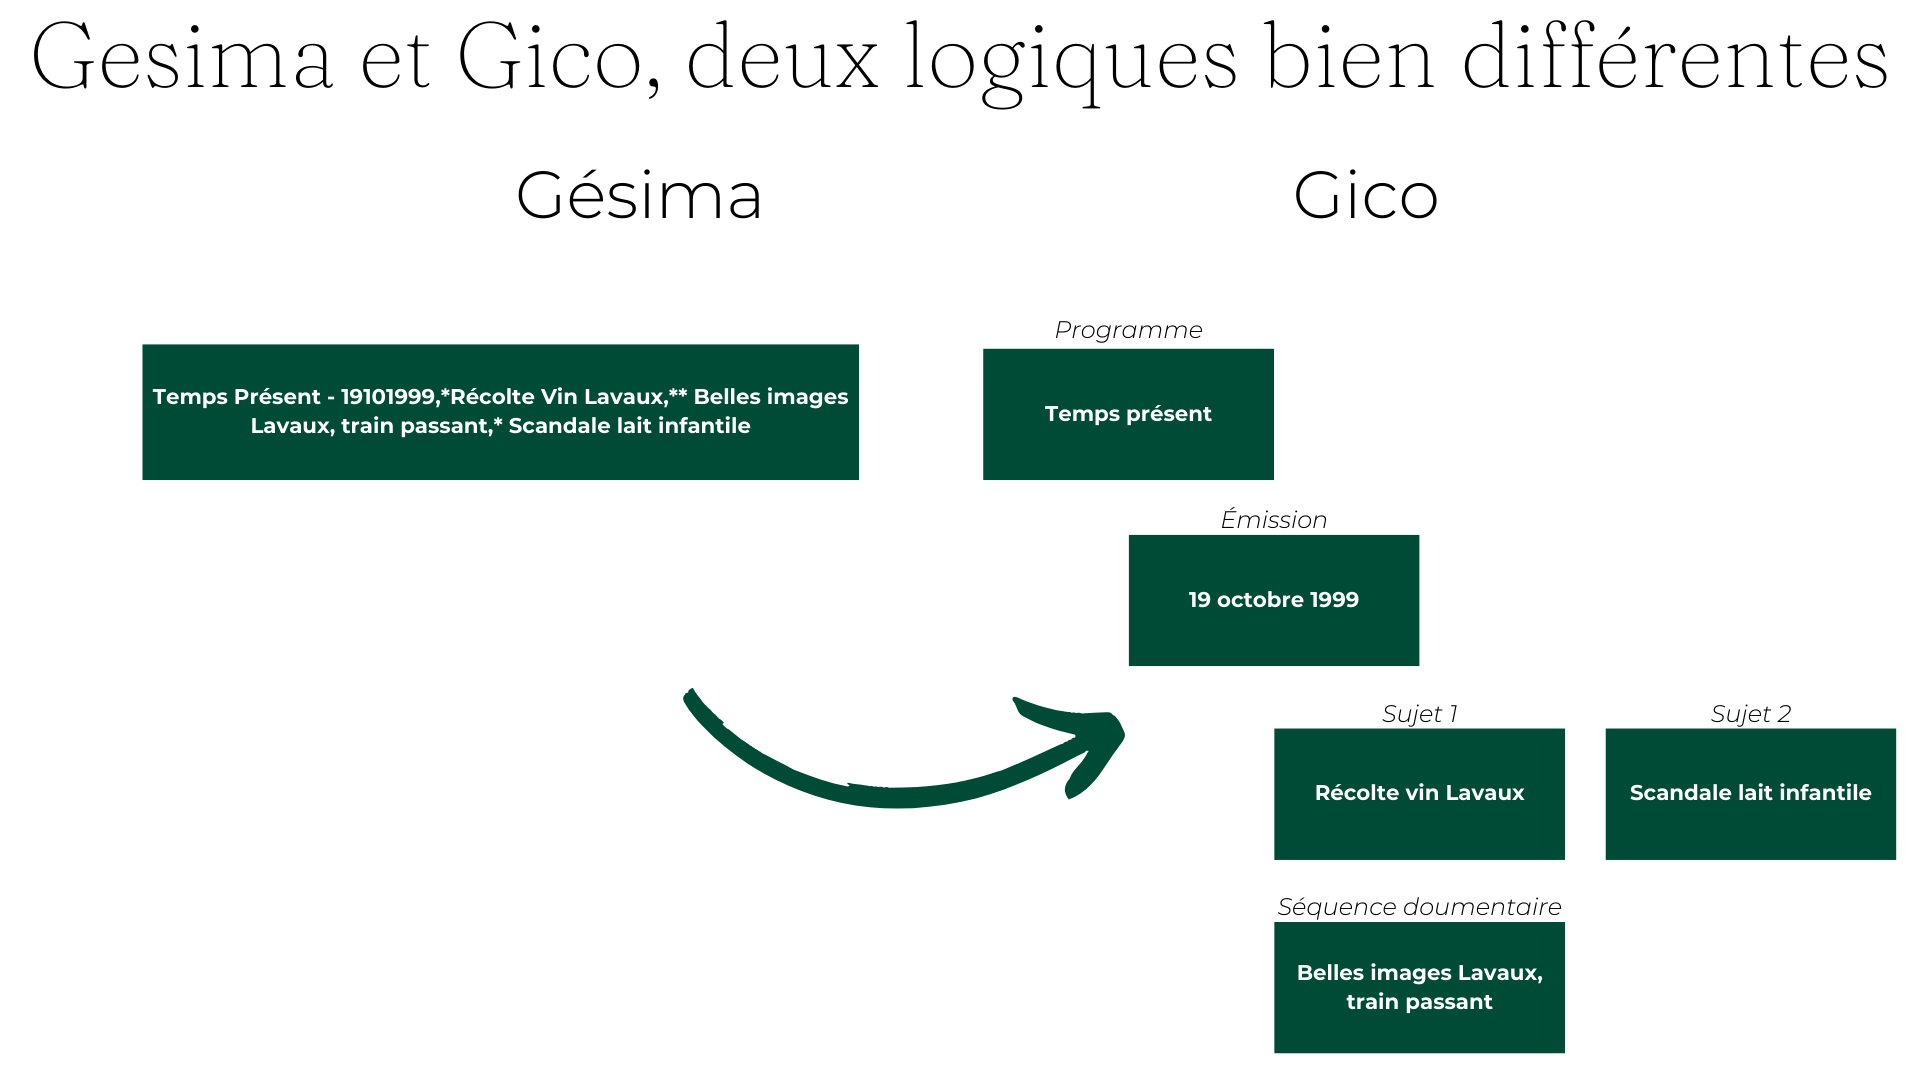
\includegraphics[width=0.8\textwidth]{images/gesimavsgico.png}
		\caption{La logique \enquote{à plat} de Gesima et la logique hiérarchique de GICO (illustration réalisée par nos soins)}
		\label{fig:image1}
	\end{figure}
	
	
	Durant le \emph{mapping}, les différentes séquences au sein d'une même émission, préalablement séparées par des astérisques sous Gesima, ont été converties en nouveaux niveaux de séquence dans GICO. Cependant, cette méthode présente des limites, notamment parce que Gesima transformait certains champs en majuscules automatiquement et limitait le nombre de caractères, rendant certaines entrées difficiles à comprendre.
	
	De plus, un problème spécifique lié à ce changement de système est que les notices importées de Gesima vers GICO contiennent souvent des doublons dans leurs résumés. Cela résulte de l'ancienne méthode de catalogage appelée "point tiret", où chaque séquence était séparée par un astérisque. Il est aussi important de noter que les dates étaient saisies de manière très variée, ajoutant un niveau supplémentaire de complexité à la gestion des données dans le nouveau système.\footcite{sonderegger2024}



\begin{figure}[h!]
	\centering
	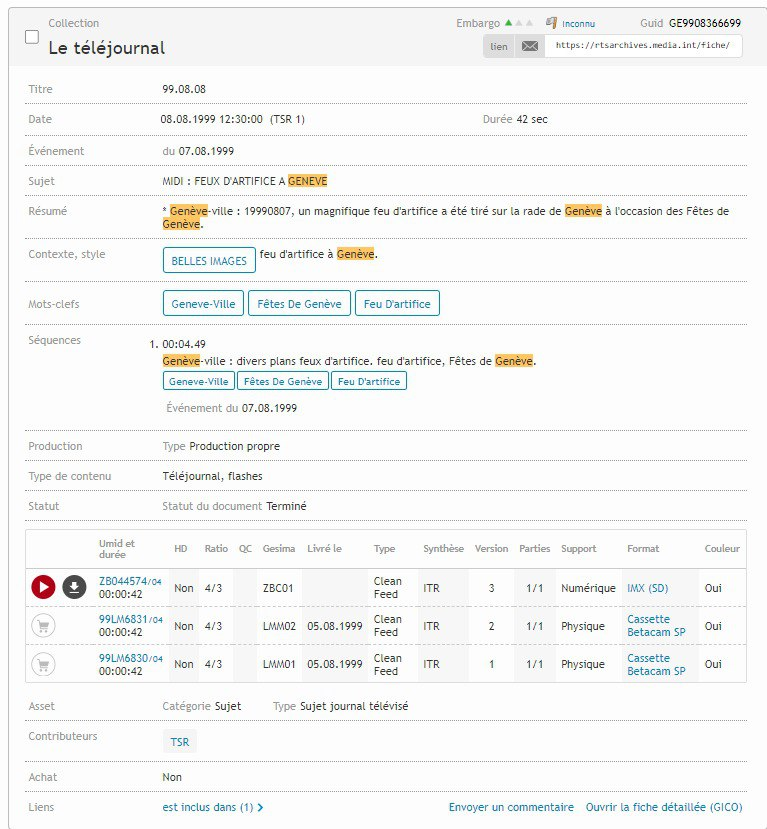
\includegraphics[width=0.8\textwidth]{images/image1.png}
	\caption{Exemple de fiche importée depuis l'outil GESIMA, on observe bien l'ancienne structuration des dates, des champs en majuscules et les problématiques que cela peut créer (information en double voire en triple)}
	\label{fig:image1}
\end{figure}


Le basculement vers GICO a permis le moissonnage de métadonnées depuis divers canaux : d’abord la possibilité de faire le lien directement avec l’image numérique archivée en base grâce à l’ajout des \textit{time code}\footnote{Un time code est un repère temporel placé sur un fichier, par exemple placé sur une séquence. Cela donne la possibilité d'y accéder de façon rapide. Par exemple si j'ai un time code à 5 minutes 33 lié à la séquences \enquote{belles images Lavaux, train passant}, un simple clic me permettra d'y accéder} ; puis en 2019 l’arrivée des données de production depuis l’outil Open Média (avec quelques problématiques d’encodage) et depuis Watson, la base de données de la programmation (notamment le sous-titrage) et enfin le lancement et la mise en production en 2022 d’outils d’intelligence artificielle\index{Intelligence artificielle|see{IA\index{IA}}} : l’un de reconnaissance des locuteurs par leurs voix, l’autre de reconnaissance faciale des personnalités passant à l’antenne\footcite{sonderegger2024}, le dernier de \textit{speech-to-text}\footnote{C'est-à-dire qui retranscrit automatiquement les paroles en texte} (mis en production en 2019). Tous ces outils ont permis de réduire considérablement le temps de description effectué par les documentalistes, mais ont aussi le défaut de générer un bruit documentaire important.


\chapter{Être repéré dans un vaste ensemble : la repérabilité}

\subsection{Naviguer dans l'océan du web : l'importance du référencement}

« Le meilleur moyen de cacher un cadavre, c’est de le mettre en page 2 des résultats sur Google »\footnote{Il est très difficile de trouver un auteur à cette citation, très présente sur le web chez les professionnels du référencement\index{Référencement}. Elle a été lue sur \url{https://www.linkedin.com/pulse/le-meilleur-endroit-pour-cacher-un-cadavre-est-\%C3\%A0-la-page-loubier-/} sans pouvoir l’attribuer avec certitude à l’auteur de l’article.}, cette phrase, quoique assez provocante, illustre assez bien l’importance pour un contenu d’être placé en tête des résultats de recherche. Pour ce faire, les professionnels de ce qu’on appelle le référencement\index{Référencement} utilisent deux stratégies : le SEO (Search Engine Optimization), l'optimisation de la page pour qu’elle soit mieux affichée dans les résultats de recherche, et le SMO (Social Media Optimization), l'optimisation du contenu sur les réseaux sociaux pour qu’il génère plus de clics et soit plus vu (on parle de facteurs sociaux). C’est là le premier enjeu autour de la repérabilité\index{Repérabilité} : pour qu’un contenu patrimonial ou un site soit repéré, il faut avant tout qu’il soit bien placé dans les résultats de recherche. Nous diviserons notre propos sur ce sujet en deux temps : d’abord « parler aux machines », où nous évoquerons les enjeux techniques spécifiques aux contenus patrimoniaux pour leur référencement\index{Référencement} ; puis « parler aux humains », où nous évoquerons les enjeux de communication et de valorisation. 

\subsection*{Parler aux machines}
« Rendre une information découvrable, dans un monde numérique, c’est la rendre accessible sous forme de données, la lier à d’autres informations pour que nos traces numériques se déploient, à l’image des réseaux de neurones dans le corps humain »\footnote{Josée Plamondon, \textit{Bien documenter pour favoriser la découverte en ligne : travailler avec les métadonnées}, rapp. tech., Canada, Fondation Jean-Pierre Perreault, 2019, \url{https://numerique.banq.qc.ca/patrimoine/details/52327/4020619}, pp. 13-14, cité dans \textit{Rapport - Mission franco-québécoise sur la découvrabilité en ligne des contenus culturels francophones}, Ministères de la Culture de la France et du Québec, France, Québec, Ministère de la Culture, 2020, p. 60, \url{https://www.culture.gouv.fr/Media/medias-creation-rapide-ne-pas-supprimer/Rapport-Mission-franco-quebecoise-sur-la-decouvrablilite-en-ligne-des-contenus-culturels-francophones.pdf}.}.

Cette citation éclaire sur l’importance de ce que nous appelons un dialogue avec les machines, qui est le premier levier vers la découvrabilité (en plus de celui de la disponibilité\index{Disponibilité} des ressources en ligne déjà mentionné). Si une ressource n’est pas visible sur les moteurs de recherche, elle aura des chances moindres d’être découverte. Il nous faut donc évoquer les enjeux techniques du référencement\index{Référencement}, et pour cela, nous devons d’abord comprendre le fonctionnement des moteurs de recherche. Nous nous focaliserons ici sur Google, car il concentre environ 90 \% de part de marché\footcite{zotero-245} et que son fonctionnement illustre celui de tous les autres moteurs de recherche. 

Ce qui a fait la popularité de Google dès sa création en 1998, c’est son algorithme (\textit{PageRank}) qui a très sensiblement amélioré les résultats des recherches sur le web d’alors, où l’habitude était plutôt d’utiliser des annuaires tels que Yahoo, car les résultats des moteurs de recherche d’alors n’étaient que peu pertinents et très facilement falsifiables. Les créateurs de sites créaient par exemple, sous leur page web, une page blanche avec des milliers d’occurrences du terme auquel ils souhaitaient être associés pour être placés en tête des résultats\footcite[§ 4]{cardon2013}.


\begin{figure}[h!]
	\centering
	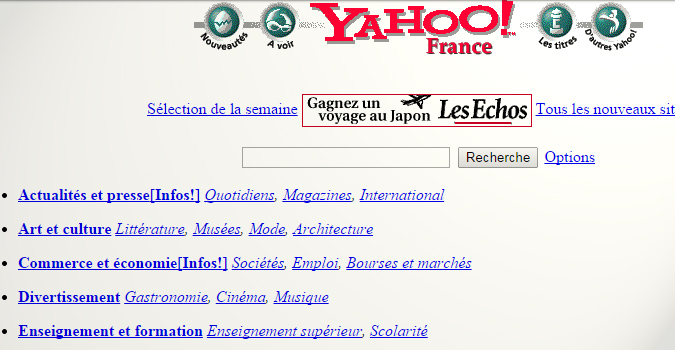
\includegraphics[width=0.4\textwidth]{images/image2.jpg}
	\caption{L'interface de Yahoo qui était au départ un annuaire }
	\label{fig:image2}
\end{figure}


L'efficacité de \textit{PageRank} est possible grâce à son utilisation d’une science inventée par Eugène Garfield : la scientométrie, au départ pour faciliter le travail des chercheurs et révéler les associations entre articles scientifiques, et les classer par nombre de citations reçues\footcite[§ 5]{cardon2013}. Traduit dans le domaine du web, plus une page a de liens pointant vers elle (on utilise souvent le terme de \textit{backlinks}), plus elle sera considérée comme centrale sur un sujet et donc pertinente. Ce principe fondamental de l’algorithme de Google a depuis été complété par un nombre impressionnant et toujours mouvant de critères, estimés à plusieurs centaines : mots-clés présents sur la page, confiance accordée au site, facteurs sociaux, temps de chargement\footcite{ertzscheid2019}… Google ne communique jamais sur ces critères afin d’éviter des pratiques d’optimisation abusives, leur conseil est toujours le même : « faites le nécessaire pour satisfaire au mieux les internautes qui visitent votre site web et ne vous préoccupez pas inutilement des algorithmes ou des paramètres utilisés par Google pour le classement »\footcite{zotero-236}. En plus de produire du contenu de qualité et utile pour les internautes, Google recommande aussi des pratiques techniques et notamment l’utilisation de « données structurées ». Pour illustrer leur importance, nous allons prendre l’exemple du projet data.bnf.fr de la Bibliothèque nationale de France (BnF).

\subsubsection{Data.bnf.fr : sortir les données du web profond}

Lancé en 2009, le projet data.bnf.fr a pour objectifs de favoriser la visibilité des données de la Bibliothèque nationale de France (BnF) sur le web ; de casser les silos que constituent les multiples catalogues de l’institution en les regroupant en un point d’entrée unique ; de « faciliter la réutilisation des métadonnées par des tiers » ; de « contribuer à la coopération et l’échange de métadonnées par la création de liens entre des ressources structurées et de confiance »\footcite{s.d.}. En bref, de « rendre les données de la Bibliothèque nationale de France plus utiles sur le web ». Pour ce faire, data.bnf.fr utilise le modèle IFLA-LRM\index{Modèles de données!IFLA-LRM} (ex. FRBR\index{Modèles de données!FRBR}) qui est structuré synthétiquement comme suit : l’œuvre d’un auteur est manifestée dans une édition, elle même matérialisée dans un item. Par exemple, \enquote{Notre-Dame de Paris} de Victor Hugo est manifesté dans une traduction anglaise qui est éditée chez \textit{Penguin Classics} et matérialisée dans un livre\footcite{bermes2023}.


\begin{figure}[h!]
	\centering
	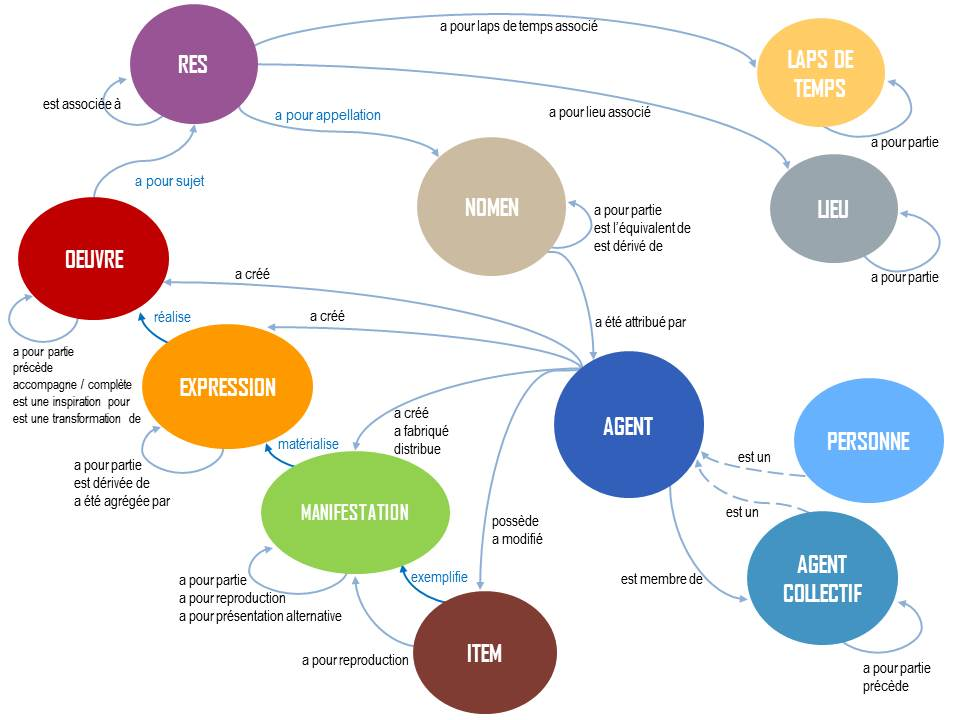
\includegraphics[width=0.8\textwidth]{images/image3.jpg}
	\caption{Illustration schématique du modèle FRBR/LRM}
	\label{fig:image3}
\end{figure}

\begin{center}
	Depuis : \url{https://data.bnf.fr/fr/semanticweb}
\end{center}



Le site (data.bnf.fr) va donc puiser dans les différentes sources de données de la BnF, qui sont dans différents formats de données : XML-EAD, Intermarc, etc. pour ensuite les structurer selon le modèle de graph-RDF (Resource Description Framework) qui est structuré en triplets : sujet, prédicat et objet. Cela donne en suivant notre exemple de tout à l’heure : Victor Hugo (sujet) a écrit (prédicat) \enquote{Notre-Dame de Paris} (objet). L’avantage d’utiliser RDF est que l’usage des triplets facilite l’interconnexion et le partage, le modèle est souvent utilisé avec des ontologies, qui sont des descriptions formelles des concepts et des relations dans un domaine particulier, afin de standardiser et structurer les données. Cela améliore l’interopérabilité\index{Interopérabilité} entre différentes bases de données et systèmes, et optimise le référencement\index{Référencement} des données sur le web, car cela rend plus claire leur structure pour un moteur de recherche\footcite{zotero-238}. Cela permet aussi de tirer partie des fonctionnalités spéciales de recherche et notamment du \textit{knowledge graph} de Google qui utilise ces triplets RDF pour créer des réseaux sémantiques d'entités et de relations, permettant à Google d'interconnecter les informations et de fournir des réponses précises et contextuelles aux utilisateurs lors de leurs recherches\footcite{google2012} (on parle de réponse zéro clic, voir figure 4 pour un exemple).


\begin{figure}[h!]
	\centering
	\begin{minipage}[b]{0.45\textwidth}
		\centering
		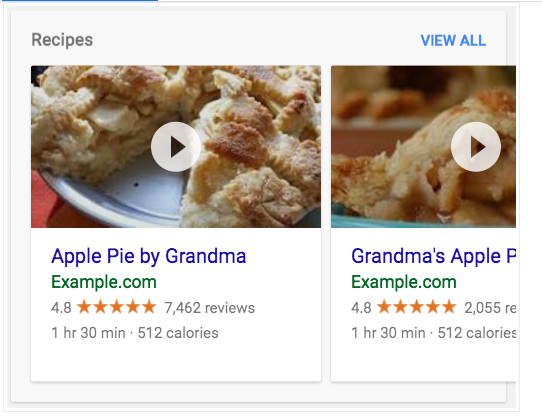
\includegraphics[width=\textwidth]{images/image4.png}
		\caption{Affichage pour l'utilisateur grâce aux données du \textit{knowledge graph}}
		\label{fig:image4}
	\end{minipage}
	\hspace{0.05\textwidth} % Espace entre les deux images
	\begin{minipage}[b]{0.45\textwidth}
		\centering
		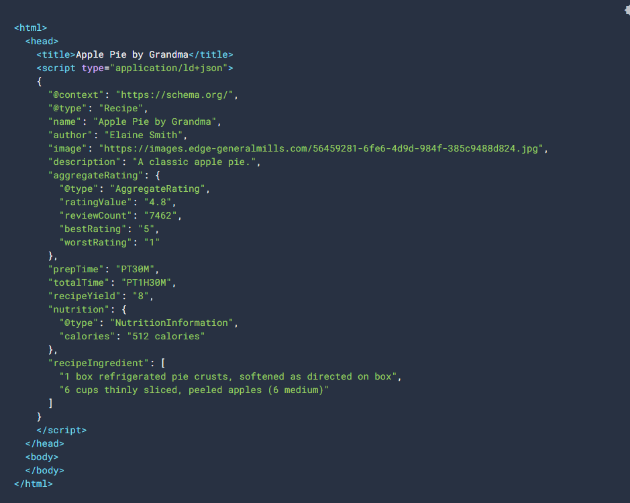
\includegraphics[width=\textwidth]{images/image5.png}
		\caption{Les données en question, affichage pour les machines}
		\label{fig:image5}
	\end{minipage}
\end{figure}
\begin{center}

Depuis :  \url{https://developers.google.com/search/docs/appearance/structured-data/intro-structured-data?hl=fr#search-appearance}

\end{center}

Par ailleurs, pour encore favoriser le référencement\index{Référencement}, data.bnf.fr utilise l’ontologie schema.org, créée justement par Google, Microsoft (Bing) et Yahoo (entre autres)\footcite{zotero-237} afin d’améliorer l’indexation des données. Le site met aussi en oeuvre son équivalent pour les réseaux sociaux, OpenGraph Protocol). De plus, data.bnf.fr expose ses données au format JSON-LD, qui permet encore d’améliorer l’indexation.\footcite{zotero-236}.

En plus de favoriser l’indexation des ressources, data.bnf.fr utilise des identifiants uniques pour chaque ressource (URI), pérennes, qui permettent aux autres bases de données de pointer vers data.bnf.fr, et inversement. Par exemple, sur Wikidata, qui est structuré selon les mêmes principes que data.bnf.fr, la page Victor Hugo pointe vers la notice du Catalogue\index{Catalogue} général de la Bibliothèque grâce à son identifiant et cette dernière pointe vers l’identifiant Wikidata de l’auteur. Outre le fait que cela génère des \textit{backlinks}, cela permet aux moteurs de recherche de comprendre que le Victor Hugo de Wikidata est le même que celui de la Bibliothèque nationale et donc de lier entre elles les données.

On l’a vu, en « parlant aux machines », data.bnf.fr a permis à ses ressources de sortir du web profond. Projet précurseur, il a été suivi par le Service interministériel des archives de France qui a lancé en 2017 le portail\index{Portail} France archives, lequel met en œuvre les mêmes principes en ajoutant la fédération des fonds sur tout le territoire (ce que fait le Catalogue\index{Catalogue} collectif de France pour la Bibliothèque nationale de France). Force est de constater que les deux projets améliorent grandement le référencement\index{Référencement}. Si je tape par exemple \enquote{capitale du Dauphiné}, c’est un extrait de Gallica qui m’est proposé par Google ; si un utilisateur fait la recherche suisnvate : « archives Simone Veil », France Archives, le portail\index{Portail} français des archives\footnote{Nous reviendrons en détails sur la question des portails dans notre partie 2}, apparaît en deuxième position derrière une communication autour de l’exposition consacrée à Simone Veil par les archives nationales.

\begin{figure}[h!]
	\begin{minipage}[b]{0.45\textwidth}
		\centering
		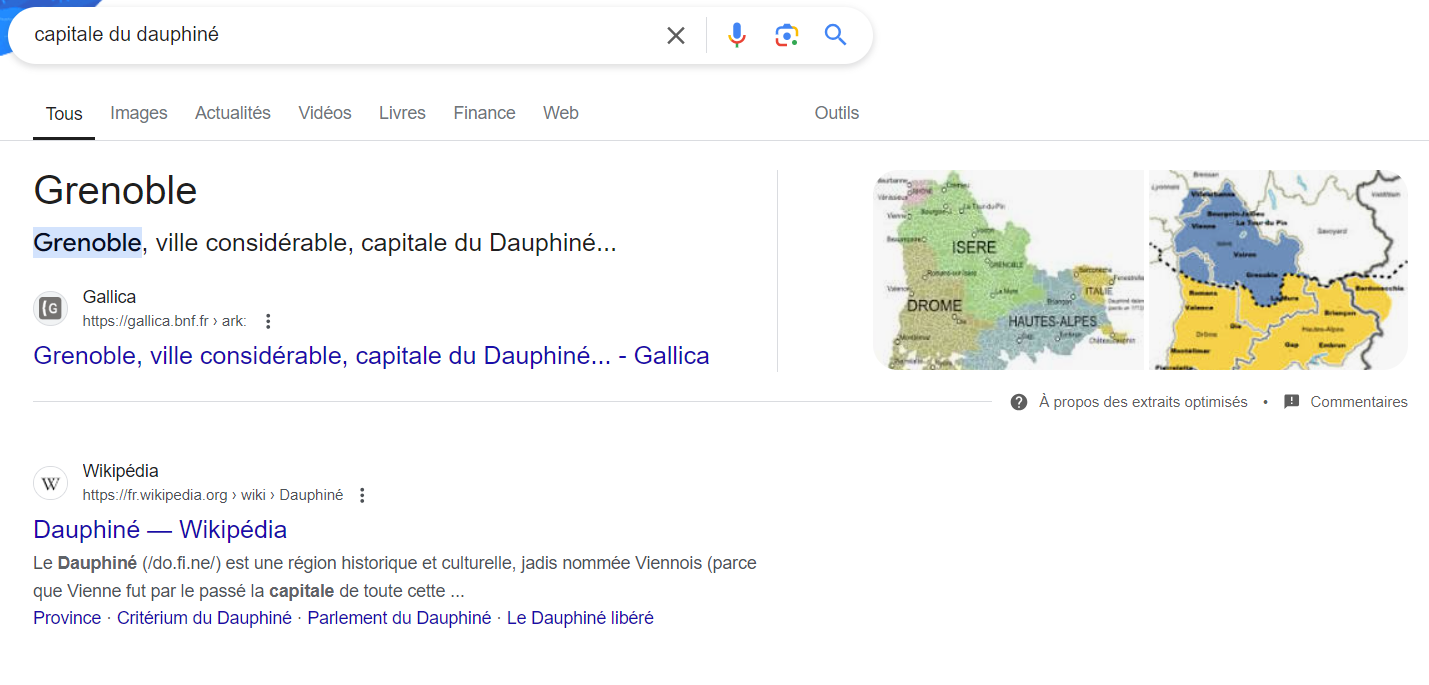
\includegraphics[width=\textwidth]{images/image7.png}
		\caption{\enquote{Capitale du Dauphiné}, résultats de recherche Google effectuée le 27 juillet 2024}
		\label{fig:image7}
	\end{minipage}
	\centering
	\hspace{0.05\textwidth} % Espace entre les deux images
	\begin{minipage}[b]{0.45\textwidth}
		\centering
		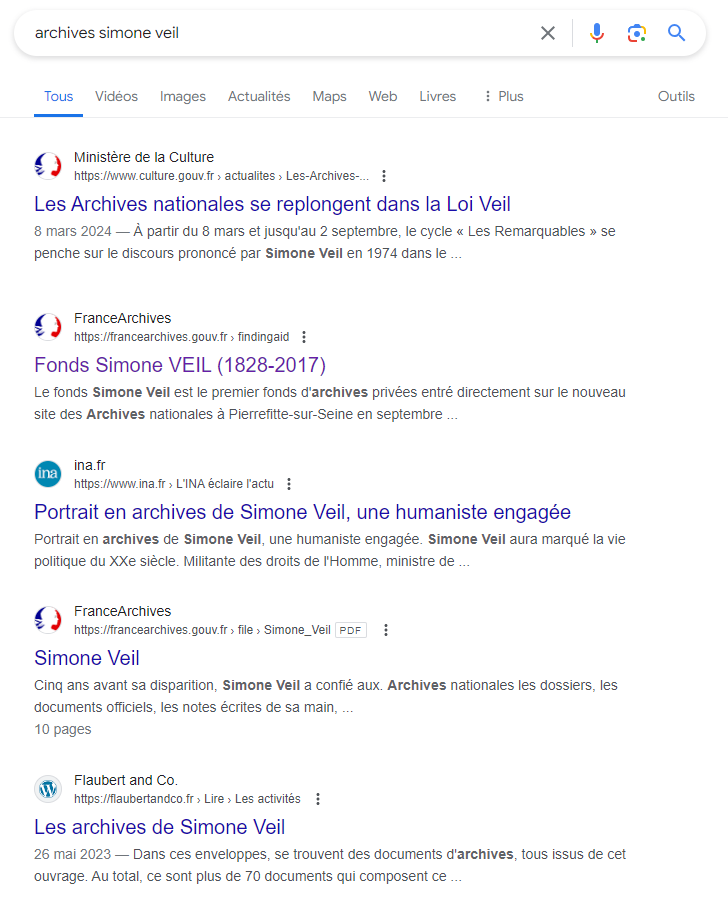
\includegraphics[width=\textwidth]{images/image6.png}
		\caption{\enquote{Archives Simone Veil}, résultats de recherche Google effectuée le 18 juillet 2024}
		\label{fig:image6}
	\end{minipage}
\end{figure}


En observant les résultats, on note deux choses : d’abord, Google génère automatiquement des réponses aux questions des utilisateurs (on parle alors de réponse zéro clic), parfois en se basant sur les données de la BnF, car les données du Knowledge graph\index{Knowledge graph} utilisées pour afficher ces questions utilisent les mêmes formats (JSON-LD)\footcite{zotero-235} que ceux mis en œuvre par data.bnf.fr, mais surtout, les deux reposent sur les principes du web sémantique. D’où une « prime » accordée à ces données dans le référencement\index{Référencement} (en plus de tout ce qui a déjà été dit). Notons aussi que le premier résultat pour notre recherche sur Simone Veil est un contenu éditorialisé « pour les humains », car tout ce que nous venons de décrire est surtout utile pour que la machine comprenne bien le contenu des pages, mais est rarement consulté réellement ; en revanche, le contenu éditorial l’est plus et ce sera l’objet de notre prochaine partie où nous détaillerons l’importance de la valorisation patrimoniale dans une stratégie de référencement\index{Référencement} en prenant l’exemple de la RTS.

\subsection{Parler aux humains : l'exemple des archives de la RTS}

Si la stratégie technique de valorisation des contenus patrimoniaux est essentielle comme décrite plus haut, car elle permet aux machines de bien comprendre le contenu et les données, cette dernière n’aurait que bien peu d’intérêt si elle n’était pas accompagnée d’une stratégie de valorisation humaine : il est inutile de bien référencer une page dont le contenu est uniquement brut. Par ailleurs, les moteurs de recherches valorisent un contenu utile et de qualité et les réseaux sociaux sont bien souvent la porte d’entrée vers les sites web tout en améliorant leur référencement\index{Référencement}\footcite{laura2022}. Dans cette partie, nous nous concentrerons sur la stratégie de valorisation des archives de la RTS, car elle nous semble rassembler les grands enjeux du domaine : un fonds au volume immense, des publics variés, et un environnement très concurrentiel.
\footnote{Josée Plamondon, Bien documenter pour favoriser la découverte en ligne : travailler avec les métadonnées, rapp. tech., Canada, Fondation Jean-Pierre Perreault, 2019, url : \url{https://numerique.
		banq.qc.ca/patrimoine/details/52327/4020619}, p. 14.cité dans : \textit{Rapport - Mission franco-québécoise sur la découvrabilité en ligne des contenus culturels francophones}, Ministères de la Culture de la France et du Québec, France, Québec, 2020, p. 60, \url{https://www.culture.gouv.fr/Media/medias-creation-rapide-ne-pas-supprimer/Rapport-Mission-franco-quebecoise-sur-la-decouvrablilite-en-ligne-des-contenus-culturels-francophones.pdf}}



\subsubsection{La \enquote{Bibliothèque de l'Honnête Homme} comme stratégie de valorisation }


Avec environ 1 million d’heures d’archives, dont les trois quarts sont audios, la RTS dispose d'une collection très riche. Cependant, ce n’est pas sans poser de problèmes, comme évoqués dans notre première partie : l’impossibilité d’appréhender dans leur totalité des objets culturels complexes générant une Fatigue muséale\index{Fatigue muséale} qu’il est difficile de contrer « much like death and taxes »\footnote{Bitgood, 2009, cité dans Windhager (Florian), Salisu (Saminu), Schreder (Günther) et Mayr (Eva), « Orchestrating Overviews : A Synoptic Approach to the Visualization of Cultural Collections », Open Library of Humanities, 4–2 (août 2018), \url{doi : 10.16995/olh.276.}}. 

Même si elle en aurait la possibilité\footnote{Hors quelques archives dont les droits ne lui appartiennent pas.}, la RTS fait le choix de ne pas donner à voir toute sa collection : ni sur le site dédié, ni sur les réseaux sociaux qu’elle anime, consciente du fait que montrer la masse documentaire presque infinie noierait les documents dits intéressants. La stratégie est donc celle d’une éditorialisation et d’une contextualisation riche, le défi est donc, comme le notent F. Windhager et al. (trad.) « de rendre les collections compréhensibles malgré une vision limitée et à des capacités d’attention restreintes »\footcite[p. 3]{windhager2018a}.

Ainsi, le site\footnote{\url{ https://www.rts.ch/archives/}} est organisé comme une « Bibliothèque de l’Honnête Homme »\footcite{chatelain2003} : suivant quelques thématiques, avec à chaque fois un nombre relativement restreint d’archives toujours éditorialisées, parfois assez sommairement, parfois de façon détaillée suivant une écriture journalistique\footnote{\url{https://www.rts.ch/archives/grands-formats/9614551-on-a-tue-bob-kennedy.html}}, favorisant le référencement\index{Référencement}. Par ailleurs, les rebonds entre différents documents sont favorisés de deux manières : leur classement dans des dossiers thématiques et les recommandations, manuelles, faites par les documentalistes (nous reviendrons en détail sur la notion de recommandation\index{Recommandation}).


\begin{figure}[h!]
	\centering
	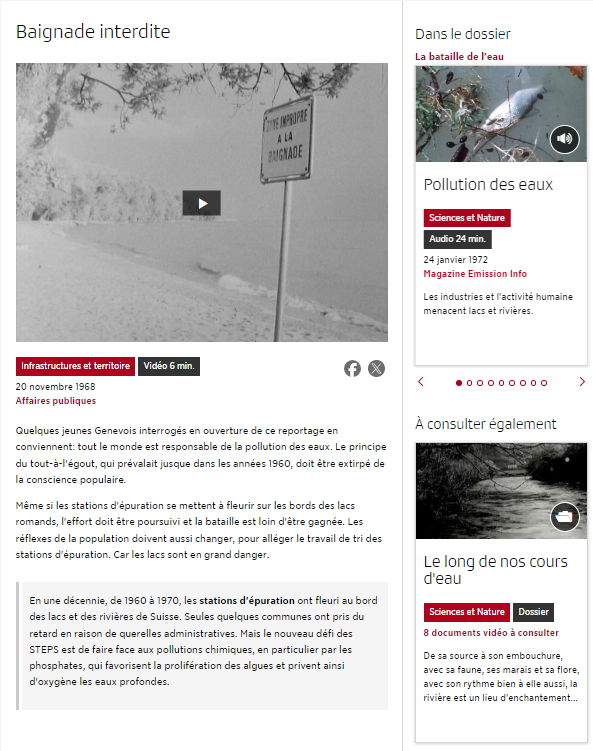
\includegraphics[width=0.8\textwidth]{images/image8.png}
	\caption{\enquote{Baignade interdite}, exemple de recommandation proposée par les documentalistes de la RTS}
	\label{fig:image8}
\end{figure}


\subsubsection{L'importance du SMO (social media optimisation)}


En 2024, sur les 5,35 milliards d’utilisateurs que compte le web, 5,04 milliards disposent d’un compte sur un réseau social\footcite{zotero-229}. Il est évident qu’il est impossible de les ignorer dans une stratégie de repérabilité\index{Repérabilité} et de référencement\index{Référencement}. C’est doublement vrai, car, d’abord — comme évoqué plus haut — une présence efficace sur les réseaux sociaux améliore le référencement\index{Référencement} dans les moteurs de recherche, on parle de SMO (social media optimisation) ; ensuite, être visible sur ces derniers génère un nombre non négligeable de clics vers les contenus, car ils représentent un tiers du temps passé en ligne\footcite{zotero-227}.

Dans le cas des archives de la RTS, ce sont clairement les réseaux sociaux qui sont le principal canal de diffusion des archives et de réception. L’institution est présente sur Facebook (490 000 followers), Instagram (115 000 followers), YouTube (607 000 abonnés), suivant la fameuse phrase de Marshall McLuhan « The medium is the message »\footcite{zotero-226} : chaque plateforme a un contenu unique et adapté. Ainsi, Instagram est alimenté en contenus courts, YouTube est le canal des formats longs, et Facebook des formats de moyenne durée. Par ailleurs, les archives sont publiées au format horizontal (plus adapté pour une consultation sur ordinateur) sur toutes les plateformes sauf Instagram, qui cible clairement un public plus jeune, sur son smartphone.


\chapter{Émerger dans le lac d'une collection : la recommandation}

\subsection{Sérendipité\index{Sérendipité} : quand l'heureux hasard rencontre les algorithmes}

« On ne trouve sans chercher que quand on a beaucoup cherché sans jamais trouver »\footcite{2015}, cette citation illustre bien le concept de sérendipité\index{Sérendipité} qui se définit comme le « don de faire par hasard des découvertes fructueuses »\footcite{zotero-224} et qui est tiré de l’anglais \textit{serendipity}, néologisme créé en 1754 par Horace Walpole à partir du conte oriental « les trois principes de Serendip », Serendip étant ici le nom ancien du Sri Lanka composé des deux mots sanscrits \textit{Sri} « souveraineté, richesse, éclat » et \textit{Lanka}, rapproché du grec \textit{lagkanein} « obtenir par le sort »\footcite{zotero-224}. La sérendipité\index{Sérendipité} serait donc, étymologiquement, l’obtention de richesses grâce au sort, mais cette définition semble réductrice par rapport à l’usage qui a été fait de ce mot. Il est en effet utilisé pour désigner des découvertes fortuites certes, mais qui ne sont jamais le total fruit du hasard. Si Flemming a découvert, par sérendipité\index{Sérendipité} (il aurait oublié des cultures de moisissures à son départ en congé), la pénicilline : c’est qu’il la cherchait ; de même, Archimède s’écriant « Euréka » dans sa baignoire alors qu’il cherchait un moyen de prouver que la couronne d’Hiéron II était composée d’or entièrement\footcite[Annexe 1]{michel2019}. Ces deux exemples illustrent le fait que la sérendipité\index{Sérendipité} est autant le fruit du hasard que de la « recherche sans jamais trouver » : c’est parce que Flemming et Archimède avaient dans leur saillance perspective\footnote{Concept sémiologique qui s’illustre bien par l’exemple suivant : à l’achat d’un vélo, on devient tout de suite très sensible à toutes les potentialités pour l’accrocher (grilles, poubelles, plots dans la rue, etc.). in Marc Jahjah, introduction à la sémiologie, cours de 1ère année de DUT information et communication, 2018 } la recherche d’une solution à leur problème.

Si au même moment, et pour les mêmes raisons que le terme de découvrabilité, le terme de sérendipité\index{Sérendipité} réémergeait en 2011, selon Francis Balle, c’est bien que les deux termes sont liés : la découvrabilité comme la sérendipité\index{Sérendipité} ne sont pas inhérentes au web, les usagers des bibliothèques le savent bien, mais tout comme la découvrabilité, en mettant au jour d’incroyables perspectives de sérendipité\index{Sérendipité} (la masse non classée permet de voir des choses inattendues), le web et ses données massives\index{Données massives} semblent aussi poser le problème. D’une navigation riche en découvertes, on peut vite se « perdre dans l’hyperespace »\footnote{Selon le livre éponyme de Quentin Quick et J. Schaherpenhuizen} et de la sérendipité\index{Sérendipité}, on passe alors à la zemblanité : où toutes les découvertes ne viennent qu’enfoncer des portes ouvertes\footcite[§ 10]{michel2019}. Il faut ici distinguer trois types de navigation sur internet : la première est celle où l’utilisateur souhaite trouver une information précise sur un sujet, il va alors saisir une équation dans un moteur de recherche, par exemple « sérendipité\index{Sérendipité} » ET « Web » (sérendipité\index{Sérendipité} quasi nulle)\footcite[p. 8]{ertzscheid2003} ; la deuxième est une navigation à proprement parler en utilisant les liens hypertextes d’une page ou d’un article (sérendipité\index{Sérendipité} structurelle)\footcite[p. 8]{ertzscheid2003} ; la troisième est basée sur l’apprentissage, l’utilisateur sait qu’il ne sait pas ce qu’il cherche (sérendipité\index{Sérendipité} associative)\footcite[p. 8]{ertzscheid2003}. Ces liens hypertextes sont l’une des spécificités d’internet, inventés en 1960 par Ted Nelson, sur base des travaux menés dès 1945 de Vannevar Bush et son Memex (il écrit dans son article « \textit{As we may think} » que le cerveau humain fonctionne par association d’idées et non de façon linéaire)\footcite{vanevarbush1945}, ils viennent casser la linéarité de lecture traditionnelle d’un texte en ajoutant des liens sémantiques activables par le lecteur\footcite{14}. Cette rupture de linéarité est un élément fondamental de la sérendipité\index{Sérendipité} sur le web, selon Olivier Ertzscheid et Gabriel Gallezot les liens hypertextes permettent « la mise en relation des unités informationnelles [...] [cela] peut permettre de découvrir des corrélations insoupçonnées »\footcite{zotero-221}. Insoupçonnées est ici un mot important, il ne s’agit jamais de hasard : ce dernier n’existe pas sur le web, les algorithmes, défini comme « suite finie et non ambigüe d’instructions et d’opérations permettant de résoudre une classe de problèmes »\footcite{2024a} rendent totalement impossible la création de hasard puisque chacune de leurs actions sont déterminées à l’avance, et même s’ils peuvent donner l’illusion de hasard (par la masse de données traitées notamment), ce dernier n’est jamais complet. Par ailleurs, il faut noter que les logiques marchandes du web, organisé en un « capitalisme linguistique »\footnote{Ce concept sera traité dans la partie 3, il est issu de l'article de Frédéric Kaplan paru dans le Monde Diplomatique en 2011 : \url{https://www.monde-diplomatique.fr/2011/11/KAPLAN/46925 }} et autour du concept d’Économie de l’attention\index{Économie de l’attention} semblent s’opposer à toute sérendipité\index{Sérendipité}.

Afin d’illustrer notre propos, prenons deux exemples, l’un tiré d’un site à but non lucratif : Wikipédia et l’autre tiré d’un site à logique marchande, Mix.com (ancien StumbleUpon). Le premier, qu’on ne présente plus, en plus de disposer d’une fonctionnalité « article aléatoire » est structuré de manière à favoriser la navigation entre les articles. Par exemple, en commençant notre lecture sur l’article « Sérendipité\index{Sérendipité} », nous avons eu connaissance d’un article écrit par Olivier Ertzscheid et Gabrielle Gallezot sur ce sujet en lien avec la recherche d’information. Connaissant préalablement bien les travaux d’Olivier Ertzscheid, nous avons décidé de consulter cet article qui s’est révélé déterminant. Wikipédia favorise donc la sérendipité\index{Sérendipité} par la présence nombreuse de liens hypertextes d’une part (sérendipité\index{Sérendipité} structurelle), mais aussi, de l’autre : par la présence des sources en bas de chaque article, souvent point de départ de fructueuses recherches.

Il nous faut en revanche présenter notre second exemple, le site Mix.com (ex-StumbleUpon). Ce dernier est basé sur un principe simple : proposer à ces utilisateurs des images/vidéos aléatoires selon leurs centres d’intérêt. Ainsi, à l’inscription sur le site, il est demandé à chaque utilisateur d’en choisir quelques-uns parmi des catégories précréées, le site lui propose ensuite une quasi-infinité d’images moissonnées depuis d’autres médias sociaux tels que Redit ou X (ex-Twitter) qu’il peut, ou non « aimer » pour que l’algorithme lui propose plus d’images du même type. Le site lui propose, dans le même temps, des images liées à ce qu’il voit.


\begin{figure}[h!]
	\centering
	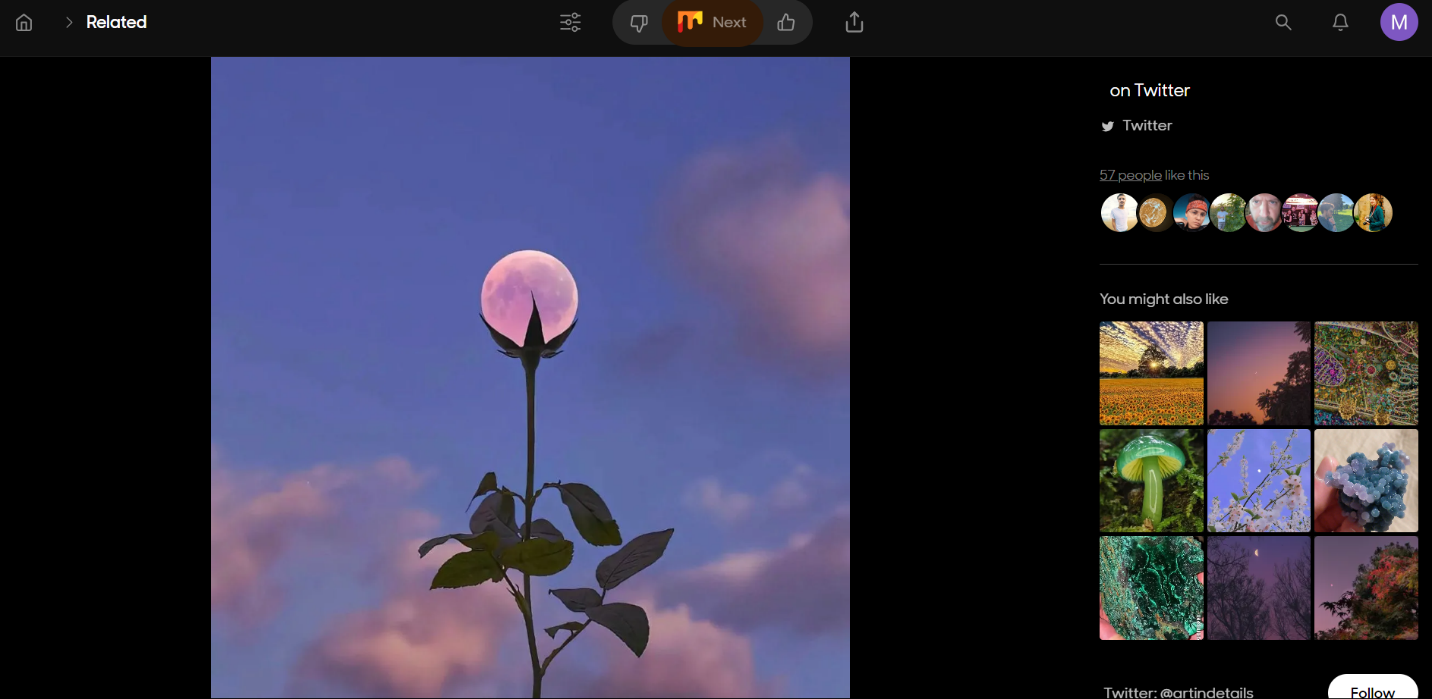
\includegraphics[width=0.8\textwidth]{images/image9.png}
	\caption{L'interface de Mix.com}
	\label{fig:image9}
\end{figure}


On a donc une sérendipité\index{Sérendipité} qui semble associative : l’utilisateur ne sait pas ce qu’il cherche, mais, à force de naviguer et d’affiner ses gouts, il finira par « tomber » sur quelque chose d’intéressant. Sauf qu’ici, le modèle économique, anciennement nommé \textit{StumbleUpon paid discovery} propose à des annonceurs de payer pour voir leur contenu propulsé à des utilisateurs, cassant ainsi le principe de sérendipité\index{Sérendipité} au profit d’une logique marchande très puissante puisque l’utilisateur croira que la publicité lui est destinée personnellement et sera bien plus enclin à la consulter : c’est tout l’intérêt des algorithmes de recommandation\index{Recommandation}\footcite{author2012}.

Finalement, de même qu’une bibliothèque par son organisation physique suivant des classifications arbitraires (citons Dewey par exemple) créé en quelque sorte une « Sérendipité\index{Sérendipité} artificielle » où les lecteurs en déambulant peuvent faire de belles découvertes, mais uniquement s’ils s’ouvrent au hasard, la sérendipité\index{Sérendipité} comme décrite par Eva Sandri va « au-delà de l’heureux hasard, il s’agirait donc d’un état de disponibilité\index{Disponibilité}, de réflexivité et d’ouverture d’esprit qui ferait en sorte de considérer l’erreur comme constructive »\footcite[p. 14]{zotero-221}. Il semble qu’on puisse conclure de la même chose pour le web : si un utilisateur s’ouvre aux heureux hasards que peut lui proposer une navigation hypertextuelle, il pourra « tomber » sur des choses intéressantes. L’immense avantage du web est qu’il n’est justement pas organisé en grandes classifications arbitraires, la navigation est donc ici interdisciplinaire « car l’internet n’a pas de frontières »\footcite[8 minutes 34 secondes]{2015} ; son immense inconvénient est en revanche les risques pour l’utilisateur de se perdre totalement dans la masse des propositions de navigation qu’il reçoit sans cesse. Les algorithmes de recommandation\index{Recommandation} peuvent alors être vus comme la solution à ce problème de la masse : en ciblant leurs utilisateurs de façon très précise et en leur proposant du contenu proche de celui qu’ils viennent de consulter, ce sont à la fois des outils de création de sérendipité\index{Sérendipité}, mais aussi des outils d’enfermement algorithmique régis parfois par des logiques marchandes (cf. exemple de Mix.com). Ils seront l’objet de notre prochaine partie.


\subsection{Les algorithmes de recommandation}



Avant toute chose, il nous faut tâcher d’expliquer le fonctionnement technique des algorithmes de recommandation\index{Recommandation}. Ces derniers ont pour objectif de rapprocher, selon des critères définis (genre, type d'utilisateur ayant regardé...), deux objets (films, musiques, textes…). Pour tâcher d’être le plus clair possible, prenons un cas d’usage : admettons que l'on souhaite rapprocher tous les programmes ayant la même thématique dans le fonds de la RTS ; nous avons pour cela à notre disposition trois choses : une transcription, un résumé et des mots-clés définis à partir d’un thésaurus. Par différentes opérations mathématiques, on va transformer ces trois éléments en un chiffre entre 0 et 1\footnote{  Dans notre cas, on utiliserait un algorithme de type TF-IDF qui calcule la fréquence (Term Frequency [TF]) d’un terme dans un document en calculant le nombre de fois où le mot apparait divisé par le nombre de mots totaux et sa rareté dans tous les documents (Inverse document Frequency [IDF]) en calculant le logarithme du nombre total de documents divisé par le nombre de documents contenant le mot, on fait ensuite TF * IDF. L’intérêt est d’identifier les mots signifiants importants pour un document en réduisant l’importance des mots vides (« le », « et »…) [Explications fournies par Chat-GPT et remaniées}. Ensuite, on place ce chiffre dans un espace vectoriel, c’est-à-dire dans un espace mathématique (voir image ci-après), le tout pour chaque archive. Les points qui sont proches sont ceux partageant des caractéristiques communes, puisque le chiffre qui a été calculé à partir de leurs métadonnées spécifiques est proche. Si l'on souhaite voir les documents (où les personnes en suivant leurs traces en ligne ou données démographiques) similaires, il suffit de prendre tous les points proches dans le graphique\footcite{zotero-216}.


\begin{figure}[h!]
	\centering
	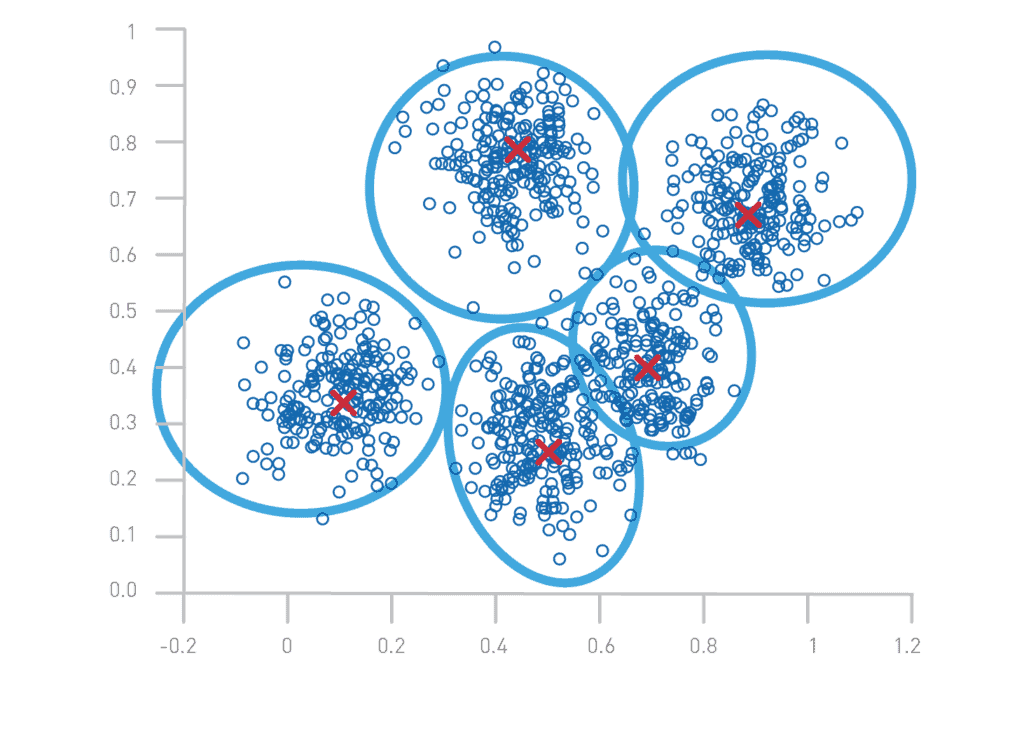
\includegraphics[width=0.8\textwidth]{images/image10.png}
	\caption{Fonctionnement schématique d'un algorithme de clustering}
	\label{fig:image10}
\end{figure}

\begin{center}
	\url{https://www.data-transitionnumerique.com/k-means/}   
\end{center}

Cette description est évidemment très simplifiée : comment délimiter les catégories entre elles ? Comment faire en sorte que mon algorithme classe tous les documents selon des thématiques définies et pas uniquement en prenant en compte, par exemple, leur champ lexical ? Mais le principe des algorithmes de Rrcommandation\index{Recommandation} est grossièrement celui décrit. Il a été expérimenté dès 1975 par Salton et al.(cité par Arnaud Claes)\footcite[p. 38]{claes2022}. En 2002, Robin Burke proposait de les répartir selon cinq catégories\footcite{claes2022} :

\begin{itemize}
	\item \textbf{Recommandation collaborative :} les contenus sont proposés en fonction des préférences de l’utilisateur et des comportements d’autres utilisateurs similaires.
	\item \textbf{Recommandation basée sur le contenu :} Les suggestions sont faites en fonction des éléments similaires consultés par l’utilisateur dans le passé.
	\item \textbf{Recommandation démographique :} les recommandations sont établies sur la base de critères démographiques tels que l’âge, le sexe et la localisation.
	\item \textbf{Recommandation basée sur un modèle de connaissance :} ces algorithmes utilisent une base de connaissances, construite grâce aux réponses de l’utilisateur à des questions spécifiques, pour suggérer des objets en fonction des besoins exprimés.
	\item \textbf{Recommandation basée sur l’utilité : }les contenus sont proposés en fonction de leur utilité pour l’utilisateur. Par exemple, si un arbre de décision pour le choix d’un produit prend en compte le coût, l’impact carbone et les notes des autres utilisateurs, un produit répondant à ces trois critères sera recommandé.
\end{itemize}

Sans rentrer dans le détail, chacune de ces catégories a des avantages et inconvénients : par exemple faire des recommandations basées sur le contenu nécessite beaucoup de données d’entraînement et de capter les traces de l’utilisateur, les recommandations basées sur l’utilité sont statiques, etc. C’est pourquoi elles sont souvent combinées, c’est par exemple le cas de Netflix qui utilise huit algorithmes différents, chacun répondant à un cas d’usage spécifique\footcite[p. 47]{claes2022}. Ce dont ces catégories témoignent, c’est aussi de deux visions : la première suppose que l’utilisateur peut explicitement donner ses préférences et la seconde, dite béhavioriste, suppose qu’il faut observer ses actions pour lui proposer du contenu\footcite[p. 38]{claes2022}. On observe clairement que la seconde vision décrite est celle qui est la plus représentée aujourd’hui, et ce, car les créateurs des algorithmes ont compris que « l’utilisateur n’est pas toujours la source la plus fiable pour éclairer ses propres intentions »\footcite[p. 39]{claes2022}. Force est de constater l’incroyable puissance de ces algorithmes quand on parle de découvrabilité, ainsi, si l’on prend l’exemple de Spotify et ses 80 millions de titres au catalogue\index{Catalogue}, on peut noter que les playlists générées par algorithme de recommandation\index{Recommandation} « découvertes de la semaine » jouent bien leur rôle. Elles auraient, en effet, permis — quelques mois après leur lancement — à quarante millions de personnes de consulter 5 milliards de morceaux nouveaux\footcite[§ 2]{durand_chapitre_2016-1}. Mais si le potentiel est immense, les enjeux le sont aussi, et notamment la transparence : comment savoir pour quelle raison tel contenu m’a été recommandé ? Surtout quand on voit à quel point les recommandations sont parfois grossières et fruits de clichés tenaces. Ainsi, en 2016, April Joyner, journaliste afro-américaine spécialisée dans les nouvelles technologies, se plaignait d’avoir vu, de façon soudaine un tiers de ses recommandations sur son compte Netflix inclure des femmes afro-américaines dans les rôles-titres et l’apparition d’une catégorie « \textit{African American Movies} » sur sa page d’accueil. Elle y voit un écueil majeur : l’invisibilisation, si l’utilisateur ne cherche pas à regarder un film de ce type et n’est pas catégorisé comme probablement de cette ethnie (April Joyner vit à Harlem\footcite{2017}), il n’en verra jamais\footnote{La question des bulles de filtre sera traitée dans la partie 3}.

On a donc des algorithmes qui, clairement, offrent un potentiel énorme de découvrabilité, mais qui, s’ils sont utilisés à des fins commerciales, finissent par réduire le champ de la découverte. Pour que les institutions patrimoniales, et plus largement les acteurs publics, puissent s’emparer du potentiel de ces algorithmes tout en évitant les problèmes posés, on a depuis quelques années vu émerger la notion d’Algorithme de service public\index{Algorithme de service public} dont nous tâcherons d’observer les différences fondamentales avec ceux mis en œuvre par les acteurs privés.



\subsubsection{La notion d'Algorithme de service public : \enquote{prenez les commandes}, l'algorithme de recommandation de Radio France}

Même si la société nationale de radiodiffusion française n’est pas un acteur patrimonial, l’ambition de son algorithme de recommandation\index{Recommandation} est comparable à ceux évoqués par Irène Bastard et Arnaud Laborderie dans un article de juin 2023 réfléchissant à la mise en place d’un tel dispositif sur Gallica, la bibliothèque numérique de la Bibliothèque nationale de France\footcite{bastard2023}. C’est-à-dire : augmenter le taux de la collection qui est consultée par les individus (48 \% sur Gallica)\footcite{bastard2023} ; améliorer les rebonds entre les items (seuls 1 à 3 documents consultés par session en moyenne sur Gallica)\footcite{bastard2023} dans des collections où il est difficile de se repérer tout en évitant les écueils des algorithmes de recommandation\index{Recommandation} commerciaux : Bulle de filtre\index{Bulle de filtre}, effets de viralité (quelques contenus reçoivent tous les clics), manque de transparence, perte de contrôle\footcite{2023b}.

Ces ambitions et craintes, pensées avec les équipes éditoriales de Radio France, ont ensuite été transformées en cinq grands principes : 
\begin{itemize}
	\item Mettre l’humain au cœur de la démarche de recommandation\index{Recommandation} ;
	\item Être totalement transparent ;
	\item Favoriser la découverte et la curiosité tout en restant efficace ;
	\item Laisser le contrôle à l’auditeur\footcite{2023b}.
\end{itemize}

La différence fondamentale avec les algorithmes de recommandation\index{Recommandation} privés est ici l’humain : il est au cœur de la démarche de recommandation\index{Recommandation} (et même de conception de cet algorithme) ; il peut comprendre pourquoi tel contenu lui a été proposé et il peut refuser qu’on l’oriente algorithmiquement et orienter l’algorithme (en lui indiquant par exemple de favoriser une émission en particulier) : le tout, pour favoriser sa découverte, car aucun humain ne pourrait naviguer dans les deux millions d’heures du catalogue\index{Catalogue} de Radio France pour recommander à chacun le programme qu’il est susceptible d’apprécier. La notion d’Algorithme de service public\index{Algorithme de service public} n’est donc pas tant technique ; certes les données d’usage (traces ou logs) collectées sont réduites ; certes aussi les algorithmes publics n’utilisent pas ou peu de données démographiques, mais ce qui est fondamentalement différent c’est qu’ils placent l’humain au cœur de leur démarche, il garde le contrôle sur ce qu’il voit, comprend pourquoi il le voit et peut décider de stopper à tout moment. Il reste donc le « pilote » de sa navigation\footcite{ertzscheid2024a}, ce qui constitue, si l’on suit l’analyse d’Olivier Ertzscheid, un retour en arrière : 
« Longtemps les technologies nous ont placées en situation de pilotage, avant de nous reléguer au rang de copilote, puis en nous laissant copilote, mais en supprimant le pilote au profit d’une seule fonction de pilotage automatique, et nous voilà désormais simplement, inexorablement, irrévocablement… passagers. Passagers par ailleurs exposés à la permanence d’un contrôle identitaire, et passagers sans autre bagage que l’acceptation naïve d’imaginer que nous pourrions encore être maitres du choix de notre destination. »\footcite{ertzscheid2024a}

Et c’est peut-être parce que Radio France est déjà un acteur majeur de la découvrabilité culturelle au travers de ses antennes que la notion d’algorithme au service du public, où l’humain est au cœur de la démarche y a été si bien comprise. Pensons par exemple à FIP (France Inter Paris), radio de l’éclectisme musical diffusant plus de 40 000 titres différents par an\footcite{2023a}, et dont le directeur écrivait en 2023 qu’il possédait le meilleur algorithme du monde : « Pourquoi ? Tout simplement, car il est humain. Chaque jour, nos programmateurs partent d’une page blanche et programment — manuellement — des tranches de vie musicale dans lesquelles toutes les musiques se doivent de se mélanger »\footcite{2023a}.


